  \documentclass[twoside=false, %  doppelseitiger Druck
    DIV=15
    ,% 11 DIV Faktor für Satzspiegelberechnung - muss bei anderen Schriftgrößen als 11pt angepasst werden , sie Doku zu KOMA Script
    BCOR=15mm, % Bindekorrektur
    headinclude=true,
    footinclude=false,
    pagesize,%         write pagesize to DVI or PDF
    fontsize=12pt,%             use this font size
    paper=a4,%          use ISO A4
%    bibliography=totoc,%         write bibliography-chapter to table of contents
    numbers=noenddot,
  ]{scrbook}

\usepackage[utf8]{inputenc}
\usepackage{makeidx}

% Fonts:
\usepackage{amsfonts}
\usepackage{lmodern}    % statt mathpazo, falls CM fonts verwendet werden sollen
\usepackage{courier}
\usepackage[scaled=.95]{helvet}
\usepackage[T1]{fontenc}
%\usepackage{mathptmx}
%\usepackage{textcomp}
\usepackage[htt]{hyphenat} % for breaking \texttt

% All in Arial Times
%\renewcommand{\rmdefault}{ptm}
%\addtokomafont{disposition}{\rmfamily}

% Math:
%\usepackage{amsmath}            % standard math notation (vectors/sets/...)
%\usepackage{bm}        % standard math notation (fonts)
%\usepackage{fixmath}        % standard math notation (fonts)

% Figures:
\usepackage{graphicx}
\usepackage{caption}
\usepackage{subcaption}
\usepackage{scrlayer-scrpage}
% \usepackage{pstool}  % einbinden falls psfrag verwendet werden soll
\usepackage{epstopdf}
\usepackage[ngerman]{babel}
\usepackage{ellipsis}  % Korrigiert den Weißraum um Auslassungspunkte
\usepackage{microtype}  % optischer Randausgleich etc.
\usepackage{acronym}
\usepackage[onehalfspacing]{setspace}
\usepackage{natbib}
\bibpunct{(}{)}{;}{a}{,}{,} %a -> Author- Year Style
\usepackage{hyperref}
\usepackage{csquotes}
\usepackage{shadethm}
\usepackage{amsthm}
\usepackage[dvipsnames]{xcolor}
\usepackage{float}
\usepackage{rotating} % turning figures
\usepackage{thmtools}
\usepackage{tcolorbox}

%code listing
\usepackage{listings}

\definecolor{darkgreen}{rgb}{0,255,0}
\renewcommand\harvardurl[1]{\textit{#1}}
\renewcommand{\lstlistingname}{Codeauflistung}
\renewcommand{\lstlistlistingname}{Quellcodeverzeichnis}
\lstset{
	inputpath={./listings/},
	frame=single,
	breaklines=true,
	captionpos=b,
	basicstyle=\footnotesize\ttfamily,
	keywordstyle=\color{blue},
	identifierstyle=\color{black},
	backgroundcolor=\color{white},
	stringstyle=\color{OliveGreen}\ttfamily,
	commentstyle=\color{gray},
	numbers=left,
	numberstyle=\tiny,
	numbersep=5pt,
	tabsize=2,
	showspaces=false,
	showtabs=false,
	xleftmargin=17pt,
	framexleftmargin=17pt,
	framexrightmargin=5pt,
	framexbottommargin=4pt,
    inputencoding = utf8,  % Input encoding
	extendedchars=true,
	showstringspaces=false,
	literate={á}{{\'a}}1  {é}{{\'e}}1  {í}{{\'i}}1 {ó}{{\'o}}1  {ú}{{\'u}}1
	{Á}{{\'A}}1  {É}{{\'E}}1  {Í}{{\'I}}1 {Ó}{{\'O}}1  {Ú}{{\'U}}1
	{à}{{\`a}}1  {è}{{\`e}}1  {ì}{{\`i}}1 {ò}{{\`o}}1  {ù}{{\`u}}1
	{À}{{\`A}}1  {È}{{\'E}}1  {Ì}{{\`I}}1 {Ò}{{\`O}}1  {Ù}{{\`U}}1
	{ä}{{\"a}}1  {ë}{{\"e}}1  {ï}{{\"i}}1 {ö}{{\"o}}1  {ü}{{\"u}}1
	{Ä}{{\"A}}1  {Ë}{{\"E}}1  {Ï}{{\"I}}1 {Ö}{{\"O}}1  {Ü}{{\"U}}1
	{â}{{\^a}}1  {ê}{{\^e}}1  {î}{{\^i}}1 {ô}{{\^o}}1  {û}{{\^u}}1
	{Â}{{\^A}}1  {Ê}{{\^E}}1  {Î}{{\^I}}1 {Ô}{{\^O}}1  {Û}{{\^U}}1
	{œ}{{\oe}}1  {Œ}{{\OE}}1  {æ}{{\ae}}1 {Æ}{{\AE}}1  {ß}{{\ss}}1
	{ç}{{\c c}}1 {Ç}{{\c C}}1 {ø}{{\o}}1  {Ø}{{\O}}1   {å}{{\r a}}1
	{Å}{{\r A}}1 {ã}{{\~a}}1  {õ}{{\~o}}1 {Ã}{{\~A}}1  {Õ}{{\~O}}1
	{ñ}{{\~n}}1  {Ñ}{{\~N}}1  {¿}{{?`}}1  {¡}{{!`}}1,
}
\lstdefinestyle{csharp}
{
	language=csh,
	morecomment=[l]{//}, %use comment-line-style!
	morecomment=[s]{/*}{*/}, %for multiline comments
	morekeywords={ abstract, event, new, struct,
		as, explicit, null, switch,
		base, extern, object, this,
		bool, false, operator, throw,
		break, finally, out, true,
		byte, fixed, override, try,
		case, float, params, typeof,
		catch, for, private, uint,
		char, foreach, protected, ulong,
		checked, goto, public, unchecked,
		class, if, readonly, unsafe,
		const, implicit, ref, ushort,
		continue, in, return, using,
		decimal, int, sbyte, virtual,
		default, interface, sealed, volatile,
		delegate, internal, short, void,
		do, is, sizeof, while,
		double, lock, stackalloc,
		else, long, static,
		enum, namespace, string,
		await, async, var},
}


\usepackage{graphicx}
\graphicspath{ {./figures/} }

\newshadetheorem{definition}{Definition}
\newtheorem*{goal}{Ziel}
\newtheorem{problem}{Problemstellung}
\newtheorem{requirement}{Anforderung}
\selectlanguage{ngerman}

\deffootnote{1em}{1em}{%
 \makebox[1em][l]{\thefootnotemark}}

\newcommand{\goalshaded}[1]{
	\begin{tcolorbox}[width=\linewidth, sharp corners=all, colback=white!95!black,boxrule=0pt]
		\begin{goal}
			#1
		\end{goal}
	\end{tcolorbox}
}
\newcommand\todo[1]{ \colorbox{yellow!30}{Todo: #1}}
\newcommand{\real}{\mathord{\mathrm{I\!R}}}
\newcommand*{\source}[1]{\tiny\par\raggedleft\footnotesize Quelle:~#1}
\newcommand*{\paragraphheader}[1]{\vspace{5mm}\noindent{\large\textbf{#1}}\\}
\newcommand{\code}[1]{\texttt{#1}}

% benötigt da \bf nicht mehr unterstützt
\DeclareOldFontCommand{\bf}{\normalfont\bfseries}{\mathbf}

\begin{document}

\pagenumbering{roman}
\selectlanguage{ngerman}

\def\figdir{figures}
\def\tabledir{tables}




\frontmatter

\pagestyle{scrplain}


\begin{titlepage}

\sffamily

\raggedleft

\vspace*{-2cm}


\includegraphics{\figdir/logo-th-rosenheim-2019_master_quer_2c.eps}

\vfill

\centering
\LARGE
% \vspace*{\fill}
%-----------
Fakultät für Informatik  \vspace{0.5cm}\\
\Large
Studiengang Informatik

\vspace{2cm}

\LARGE

Erstellung einer standardisierten Material-Kostengliederung für Projekte einer Bausoftware mittles Natural Language Processing

\vspace{2cm}

\Large
Bachelor Thesis

\vspace{1.5cm}


\Large
von

\vspace{0.5cm}

%\vspace*{\fill}

\LARGE
Florian Weidner \vspace{1cm}

\vspace{1cm}

\flushleft
 \Large
\vspace*{\fill}

%-----------
\begin{tabbing}
Datum der Abgabe: \= tt.mm.jjjj \kill
Datum der Abgabe: \> tt.mm.jjjj \\
Erstprüfer: \> Prof.\ Dr.\  Marcel Tilly\\
Zweitprüfer: \> Prof.\ Dr.\ Johannes Jurgovsky
\end{tabbing}
%-----------

\end{titlepage}

\cleardoubleemptypage

{
\large
\thispagestyle{empty}
\vspace*{\fill}

\noindent
\textsc{Eigenständigkeitserklärung / Declaration of Originality}

\medskip

\noindent
Hiermit bestätige ich, dass ich die vorliegende Arbeit selbständig verfasst und keine anderen als die angegebenen Hilfsmittel benutzt habe. Die Stellen der Arbeit, die dem Wortlaut oder dem Sinn nach anderen Werken (dazu zählen auch Internetquellen) entnommen sind, wurden unter Angabe der Quelle kenntlich gemacht.

\medskip

\textit{I declare that I have authored this thesis independently, that I have not used other than the declared sources / resources, and that I have explicitly marked all material which has been quoted either literally or by content from the used sources.}

\bigskip

\noindent
Rosenheim, den tt.mm.jjjj

\vspace*{2cm}

\noindent
Vor- und Zuname
}

%%% Local Variables: 
%%% mode: latex
%%% TeX-master: "d"
%%% End: 

\cleardoubleemptypage

\chapter*{Abstract}
Anhand der vorliegenden wissenschaftlichen Arbeit sollte ein Konzept für die hierarchische Strukturierung von Materialien aus \acf{ifc}-Dateien für eine Programmerweiterung der Bausoftware ORCA AVA erarbeitet werden. Dafür sollen passende \acf{nlp}-Algorithmen für die Strukturierung ausgewählt werden. Es wurden verschiedene Algorithmen nach definierten Kriterien der Messbarkeit evaluiert und passende ausgewählt. Materialangaben bestehen meistens aus Stichpunkten mit nur einem oder wenigen Wörtern und fallen somit in die Kurztext-Klassifizierung. Zusätzlich müssen Fachbegriffe richtige verarbeitet werden. Die Materialstrukturierung wurde in die Textklassifizierung und eine weitere Feinstrukturierung aufgeteilt. Für die Textklassifizierung stellte sich ein Maximum Entropy Model mit dem \ac{sdca}-Optimierungsalgorithmus trotz Kurztext-Klassifizierung mit einer Genauigkeit von 88,2 \% als beste Wahl heraus. Bei der Feinstrukturierung wird eine domänenspezifisches \textit{fastText}-Modell trainiert, um die Bedeutung der Wörter, trotz Stichpunkte und Fachbegriffen, bei der Vektorisierung der Materialien mitzugeben. So können die Materialien mit \acf{dbscan}-Clustering weiter strukturiert werden. Dieses Vorgehen schneidet besser ab, als das Nutzen des ChatGPT-Modells von OpenAI. Für das Ausführen der Strukturierung wurde ein Webservice implementiert, um die Machine-Learning-Modelle zentral nutzen zu können und keine Pythonumgebung für die ORCA AVA installiert werden muss.\\

\noindent Schlagworte: \acs{nlp}, Machine Learning, \acs{ifc}, \acs{bim}, ML.NET, fastText, \acs{dbscan}


\cleardoubleemptypage


\tableofcontents
\clearpage
\listoffigures
%\clearpage
%\listoftables
\cleardoublepage

\addtokomafont{caption}{\small}
\mainmatter

\begin{onehalfspace}
\section{Motivation}
\subsection{Problemstellung}
\label{s:intro}
Das übergeordnete Ziel für die Bausoftware ORCA AVA ist es, möglichst viele Informationen aus 3D-Modellen von Gebäuden in der Ausschreibungssoftware automatisch importieren zu können. Das spart dem Architekten am Anfang in der Ausschreibung viel Zeit. Der für die Bachelorarbeit relevante Teil ist die Übernahme der Baustoffe und Materialien des Objektes/Bauteils. Aus dem Modell übernommene Bauteile sollen also automatisch einer im vor hinein generierten Material-Kostengliederung zugewiesen werden.
Als öffentliches Standardformat für 3D-Gebäudemodelle gibt es IFC, welches auch in der ORCA AVA benutzt wird. In diesen Modellen können auch die Materialien der einzelnen Bauteile spezifiziert werden. Diese können an verschiedenen Stellen an einem Bauteil im Modell angegeben werden. Für Materialbezeichnungen gibt es auch keine richtigen Standards. Hier besteht das Problem, dass das Textfeldern für die Materialangabe ein offenes Textfeld ist und somit keine feste Vorgabe existiert und jedes IFC-Modell anders strukturiert ist. Deswegen ist das Ergebnis jeder Kostengliederung unterschiedlich und vom jeweiligen Modell abhängig.

\subsection{Ziel}
Ziel ist es eine Kostengliederungsstruktur in der Bausoftware ORCA AVA aus den Materialeininformationen einer IFC-Datei zu generieren. Diese Kostengliederung kann am Anfang eines Projektes einmal importiert werden. Wenn dann im Laufe des Ausschreibungsprozesses ein Bauteil aus der IFC-Datei in die ORCA AVA übernommen wird, soll es automatisch einem Material in dieser Kostengliederungsstruktur zugewiesen werden. So kann man das ausgeschriebene Gebäude nach den Materialangaben sortieren und auswerten.
\\


Ein Algorithmus soll zuerst die Möglichkeiten der Materialangabe in der IFC-Datei zusammenführen. Mit Hilfe von Natural Language Processing und Artificial Inteligence eine Lösung entwickelt werden, um einen klassifizierten und standardisierten Materialbaum zu erschaffen. Dieser Baum muss am Ende in das schon von ORCA vorhandene Format einer Kostengliederung abgebildet werden.


\section{Ausgangslage}

Das Projekt basiert vor allem auf das Themengebiet von Natural Language Processing (NLP). Mit Algorithmen wie WordNet oder Textklassifizierungen.

Innerhalb der Firma gibt es noch fast kein Wissen über dieses Themengebiet. Das Projekt ist also hier ein Test um Themen wie maschinelles Lernen oder NLP in die Entwicklung zu integrieren.

Für das Auslesen von IFC-Dateien wird das Open Source Framework XBim verwendet. Über diese Schnittstelle können die einzelnen Positionen der möglichen Materialangabe ausgelesen und dann zusammengeführt werden. Auf der anderen Seite sind die Abbildungen einer Kostengliederung schon vorhanden. Diese ist eine simple Baumstruktur, die die Oberfläche anzeigen und anpassen kann.
Technisch ist gewünscht, dass das Projekt in CSharp zu implementieren ist. Es dürfen zusätzlich auch Python-Skripte verwendet werden.

\section{Kriterien der Messbarkeit}

Um verschiedene Methoden vergleichen zu können, sind Kriterien notwendig an welchen die Methoden verglichen werden. Beim Vergleich verschiedener Maschine Learning Algorithmen sind vor allem folgende Kriterien wichtig:
\begin{description}
	\item[-] Genauigkeit des Algorithmus durch Testdaten
	\item[-] Interpretierbarkeit des Algorithmus
	\item[-] Skalierbarkeit des Algorithmus 
	\item[-] Robustheit des Algorithmus \cite{mic-ml-comparison}
\end{description}


Aspekte wie Geschwindigkeit und Ressourcenbedarf spielen eine sekundäre Rolle. Da die Anwendung eine Desktop-Applikation ist, sollte Performance kein Problem geben. Wenn der analysierte Algorithmus den Anwendungsfluss sehr beeinträchtigt und verlangsamt, scheidet er als Option allerdings aus.
Das Endergebnis der Material-Kostengliederungen aus verschiedenen Projekten, werden fachlich vom Produktmanagement bewertet. Diese habe das fachliche Wissen, um das Ergebnis bewerten zu können.

\section{Vorläufige Gliederung}
Siehe Seite 5 und 6.
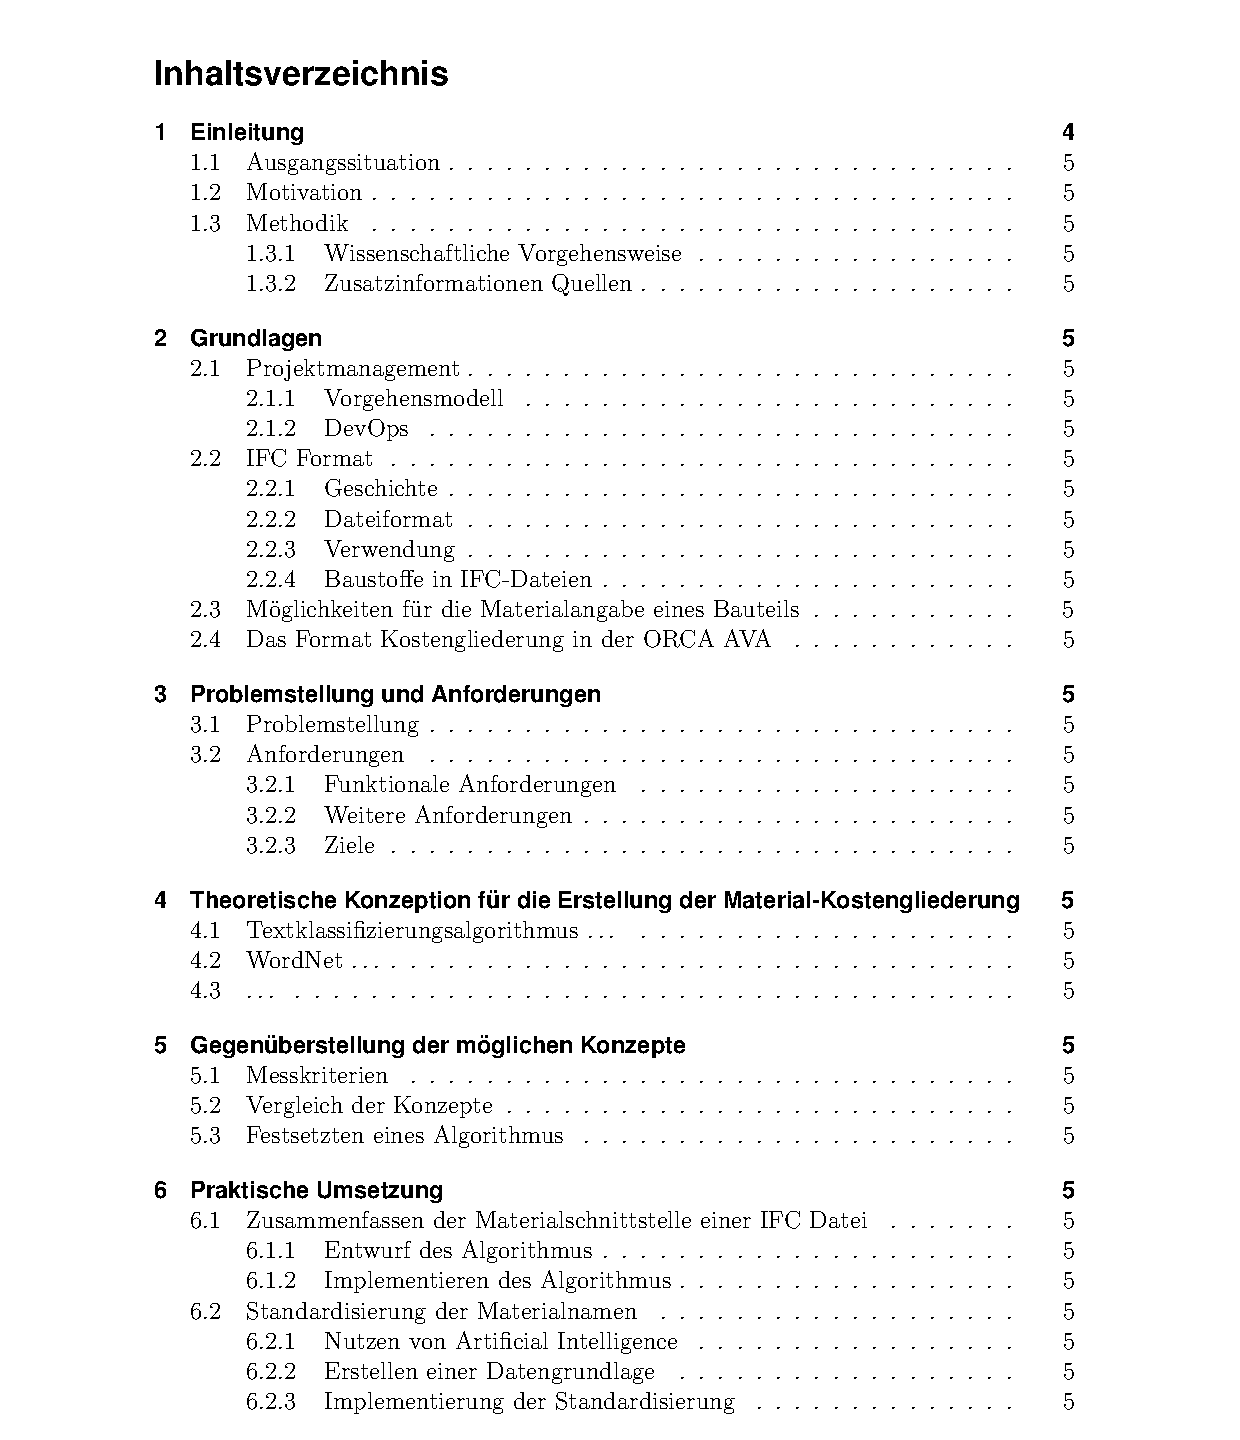
\includepdf[pages=-]{figures/inhaltsverzeichnis.pdf}
\section{Zeitplan}

\begin{description}
	\item[1.]
	Recherchieren über verschiedene mögliche Techniken und Algorithmen (2 Wochen)
	\item[2.] 
	Austesten der gefundenen Algorithmen (2 Wochen)
	\item[3.]
	Messen der Ergebnisse der Algorithmen (1 Wochen)
	\item[4.] Implementieren des besten Ergebnisses (1 Wochen)
	\item[5.] Schreiben der Arbeit (ca. 6 Wochen)
\end{description}

%\section{Erste Literatur}

%Für IFC gibt es von buildingSMART eine technische Beschreibung der Schnittstelle. Diese hilft die möglichen Materialangaben zu lokalisieren und zusammenfügen zu können. \cite{security-model}
\end{onehalfspace}

\appendix

\chapter{Anhang}
\label{a:append}
\section*{Abbildungen}

\begin{figure}[H]
	\centering
	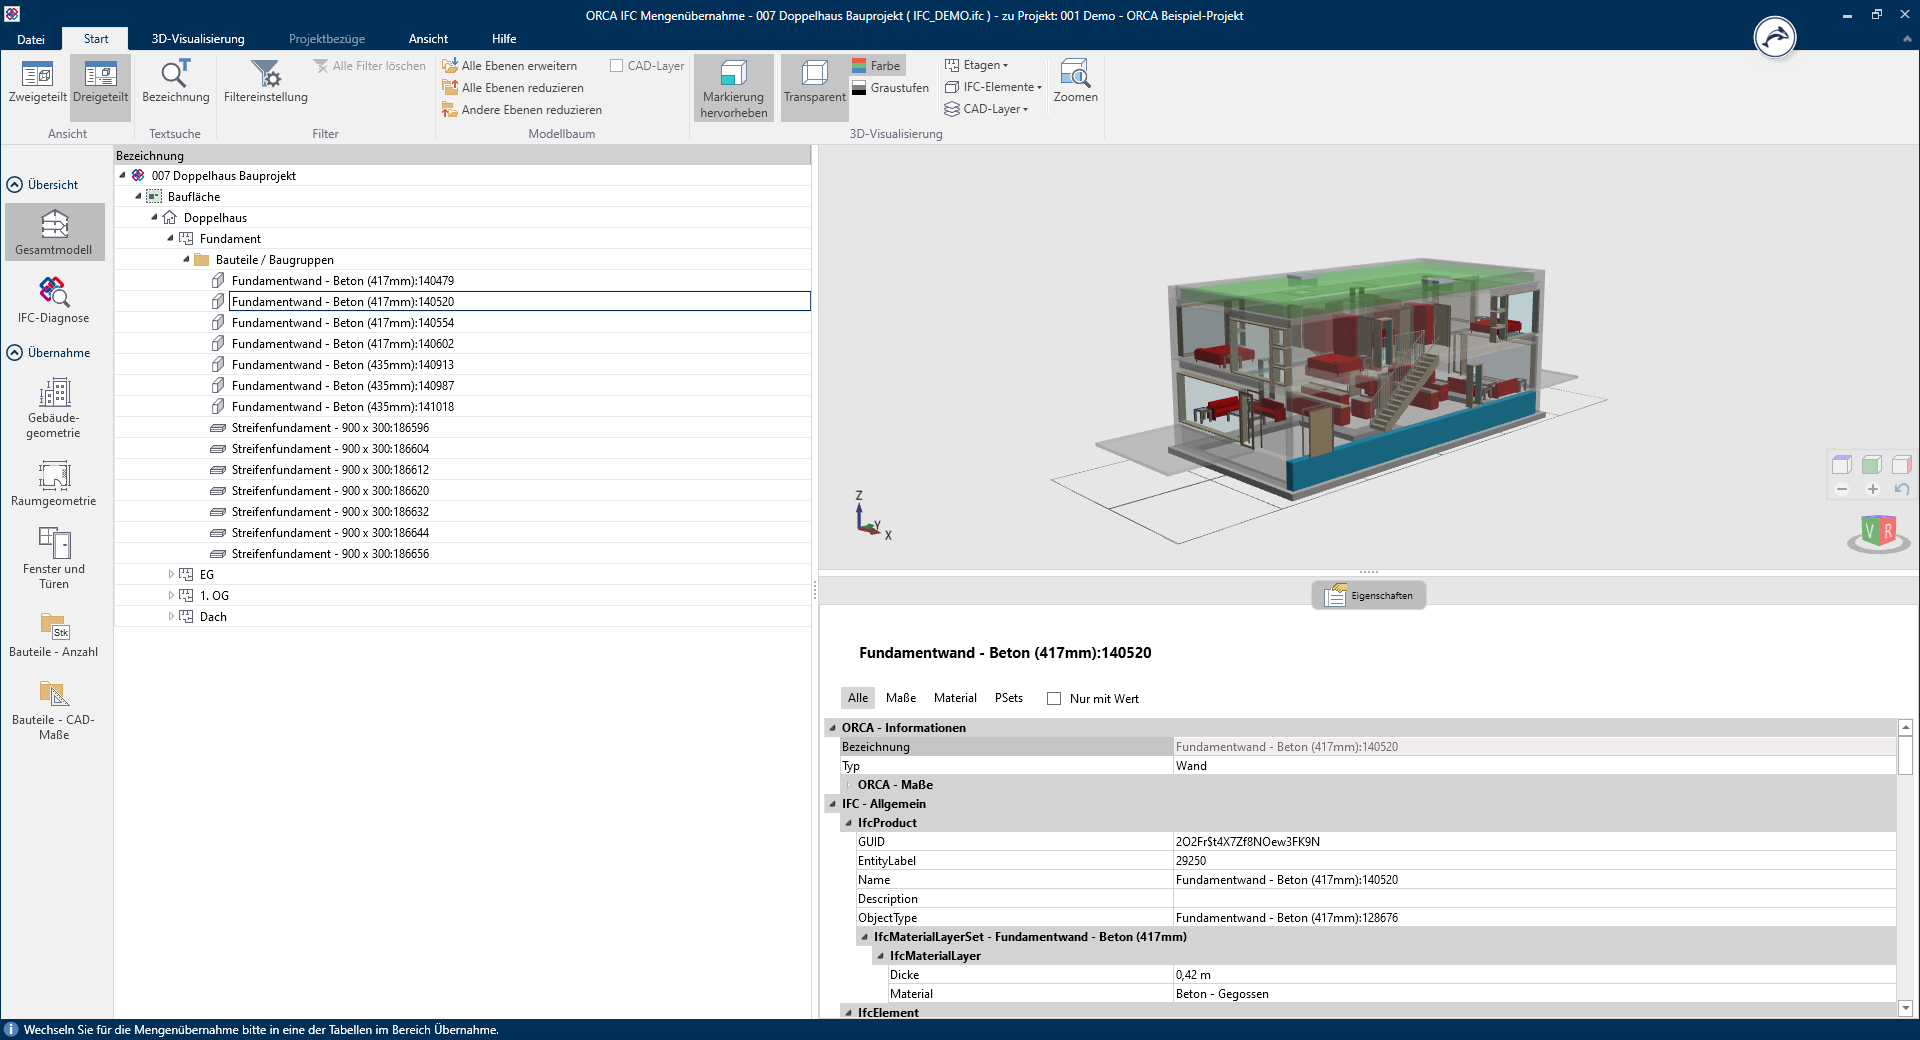
\includegraphics[width=1\linewidth]{ifc-manager}
	\caption[IFC Manager]{Oberfläche des \ac{ifc} Manager}
	\label{fig:ifc-manager}
\end{figure}

\begin{figure}[H]
	\centering
	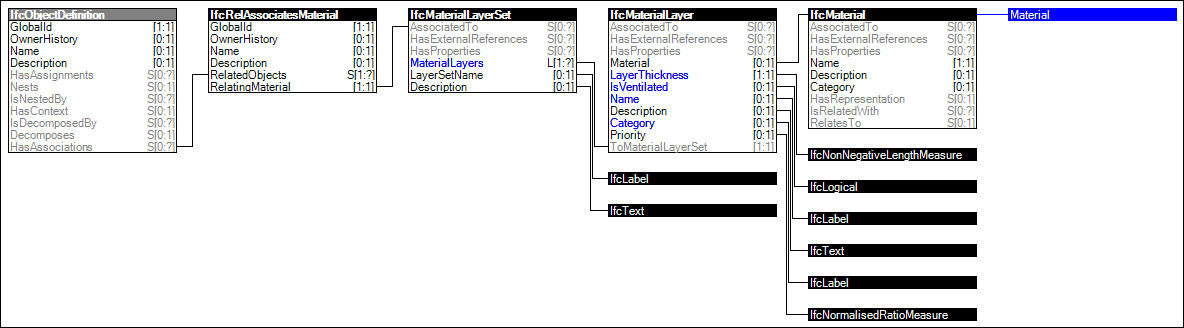
\includegraphics[width=1\linewidth]{material-layer-set}
	\caption[IfcMaterialLayerSet]{Material Layer Set Association}
	\label{fig:layer-set}
\end{figure}

\begin{sidewaysfigure}
	\centering
	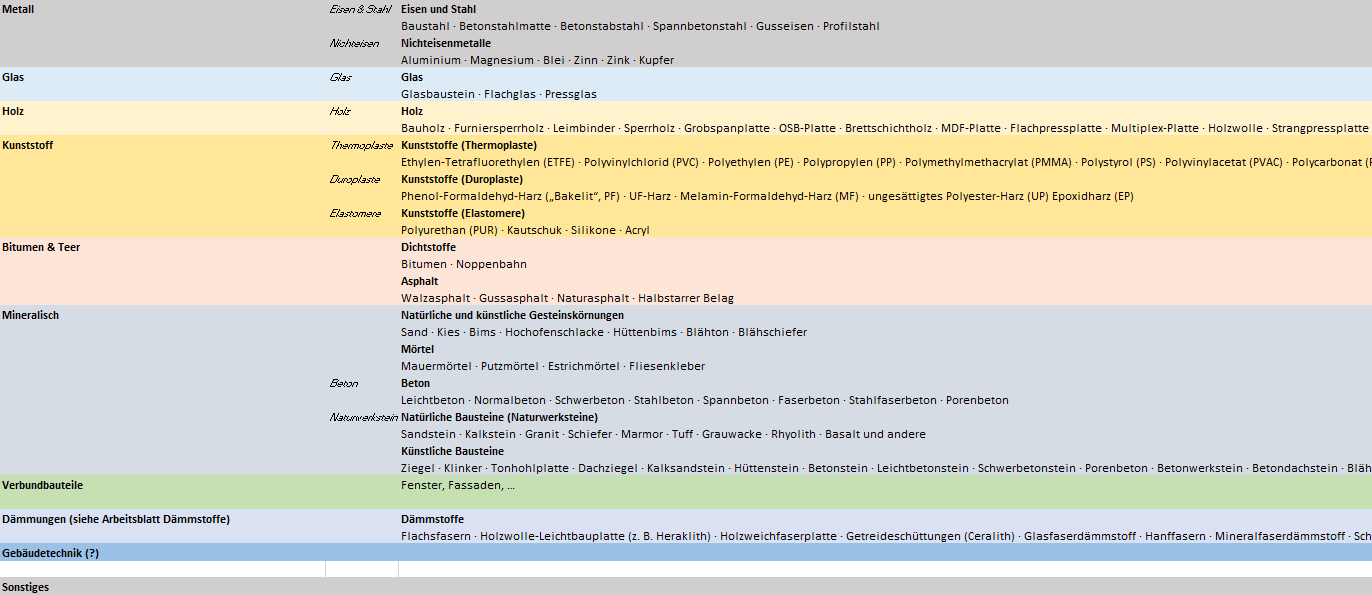
\includegraphics[width=\textheight]{material-categories}
	\caption[MaterialCategories]{Überkategorien für die Klassifizierung von Materialien mit Beispielen}
	\label{fig:material-categories}
\end{sidewaysfigure}

\begin{figure}[H]
	\centering
	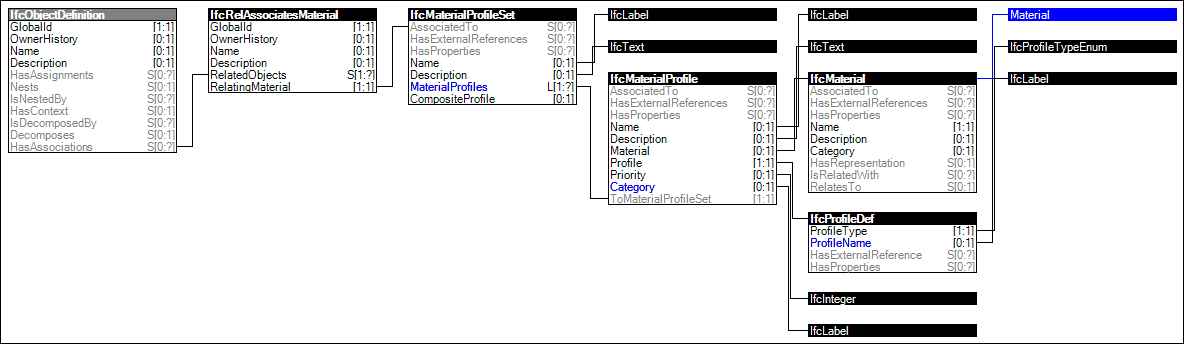
\includegraphics[width=1\linewidth]{material-profile-set}
	\caption[IfcMaterialProfileSet]{Material Profile Set Association}
	\label{fig:profile-set}
\end{figure}

\begin{figure}[H]
	\centering
	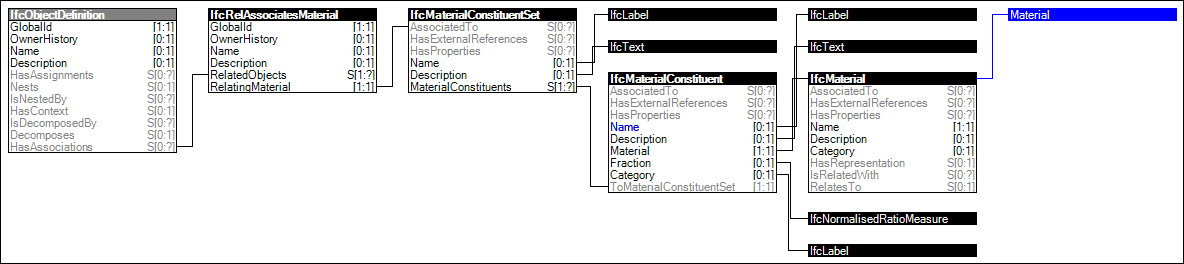
\includegraphics[width=1\linewidth]{material-constituent-set}
	\caption[IfcMaterialConsituentSet]{Material Constituent Set Association}
	\label{fig:constituent-set}
\end{figure}

\begin{figure}[H]
	\centering
	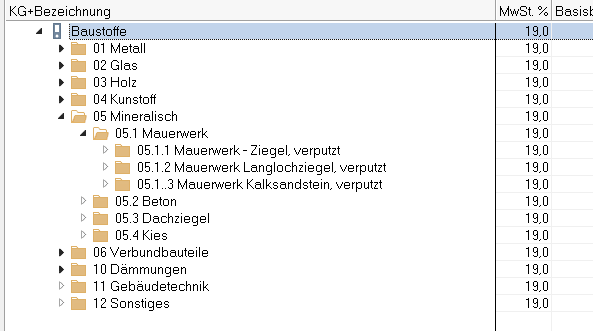
\includegraphics[width=1\linewidth]{cost-structure-example}
	\caption[CostStructure]{Beispiel einer Kostengliederung in der ORCA AVA}
	\label{fig:cost-structure}
\end{figure}

\begin{figure}[H]
	\centering
	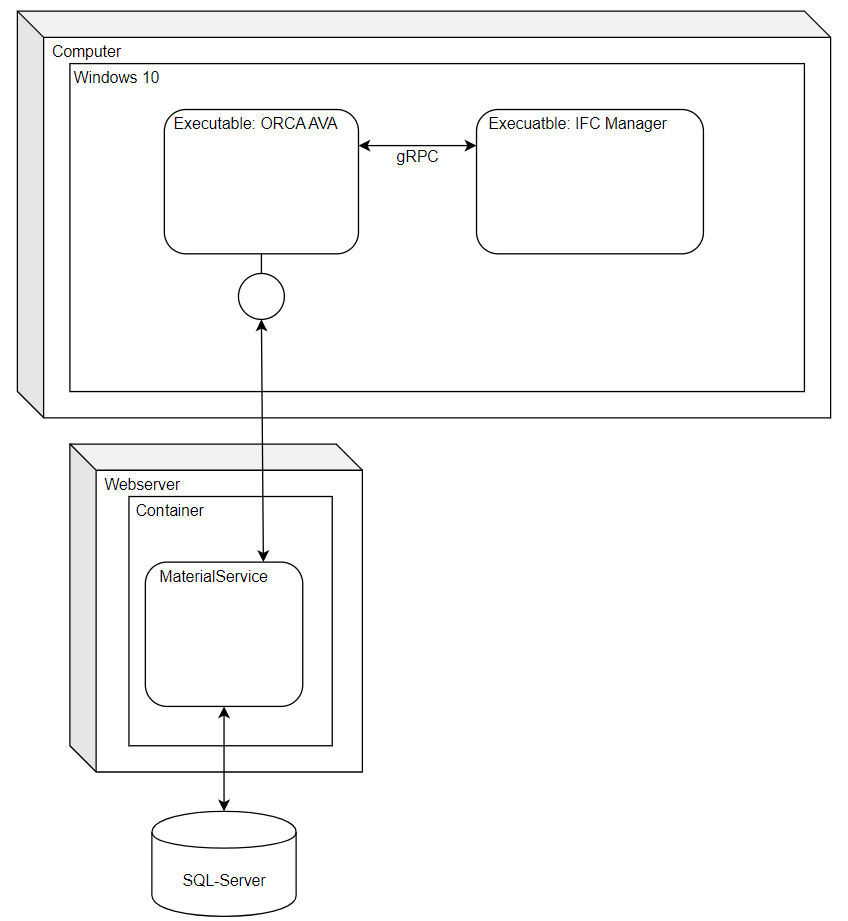
\includegraphics[width=1\linewidth]{verteilungsdiagramm}
	\caption[Verteilungsdiagramm]{Verteilungsdiagramm der Architektur}
	\label{fig:distribution-diagramm}
\end{figure}

\begin{figure}[H]
	\centering
	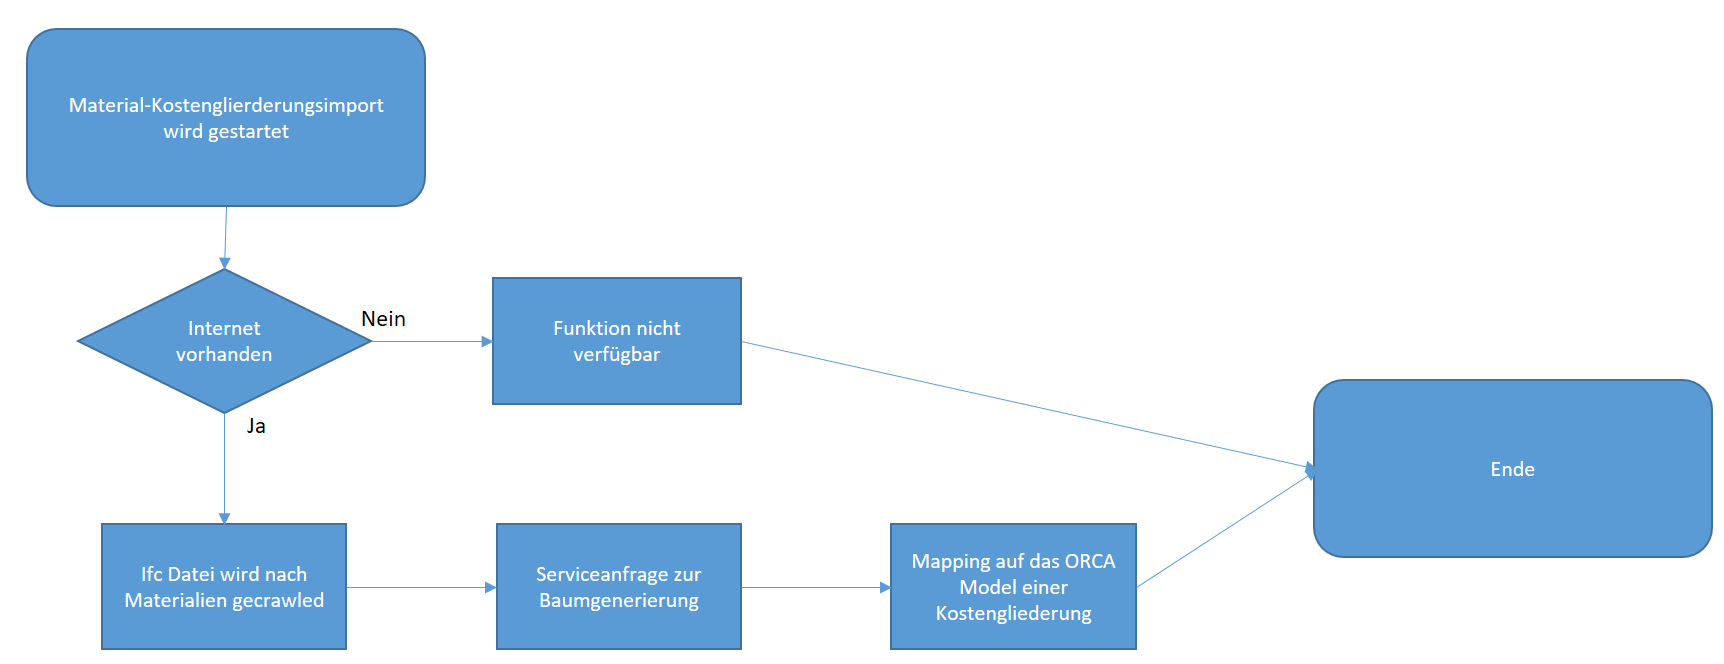
\includegraphics[width=1\linewidth]{function-import}
	\caption[Import]{Flussdiagramm Import der Material-Kostengliederung}
	\label{fig:func-import}
\end{figure}

\begin{figure}[H]
	\centering
	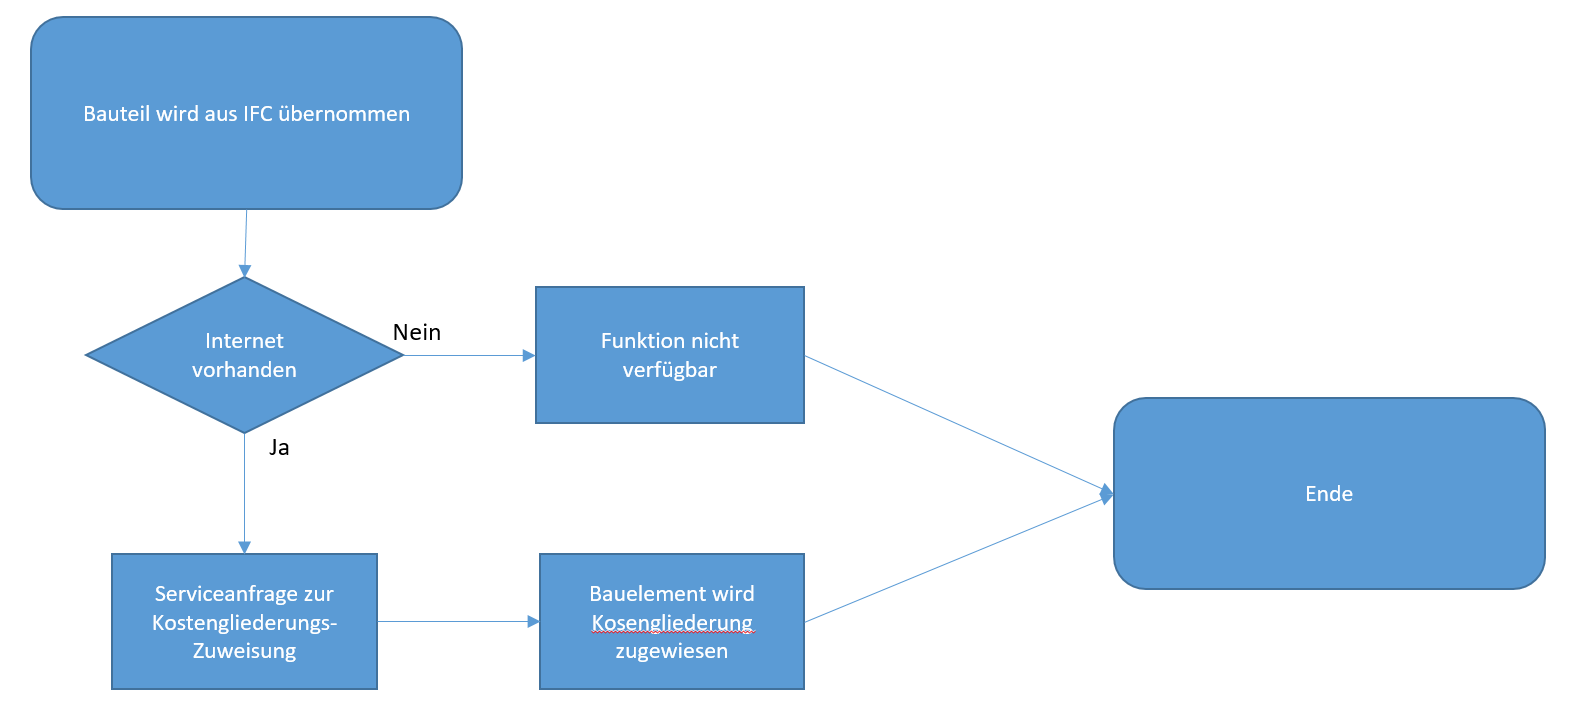
\includegraphics[width=1\linewidth]{function-takeover}
	\caption[Takeover]{Flussdiagramm Übernahme von Mengen aus dem \ac{ifc} Manager}
	\label{fig:func-takeover}
\end{figure}

\begin{figure}[H]
	\centering
	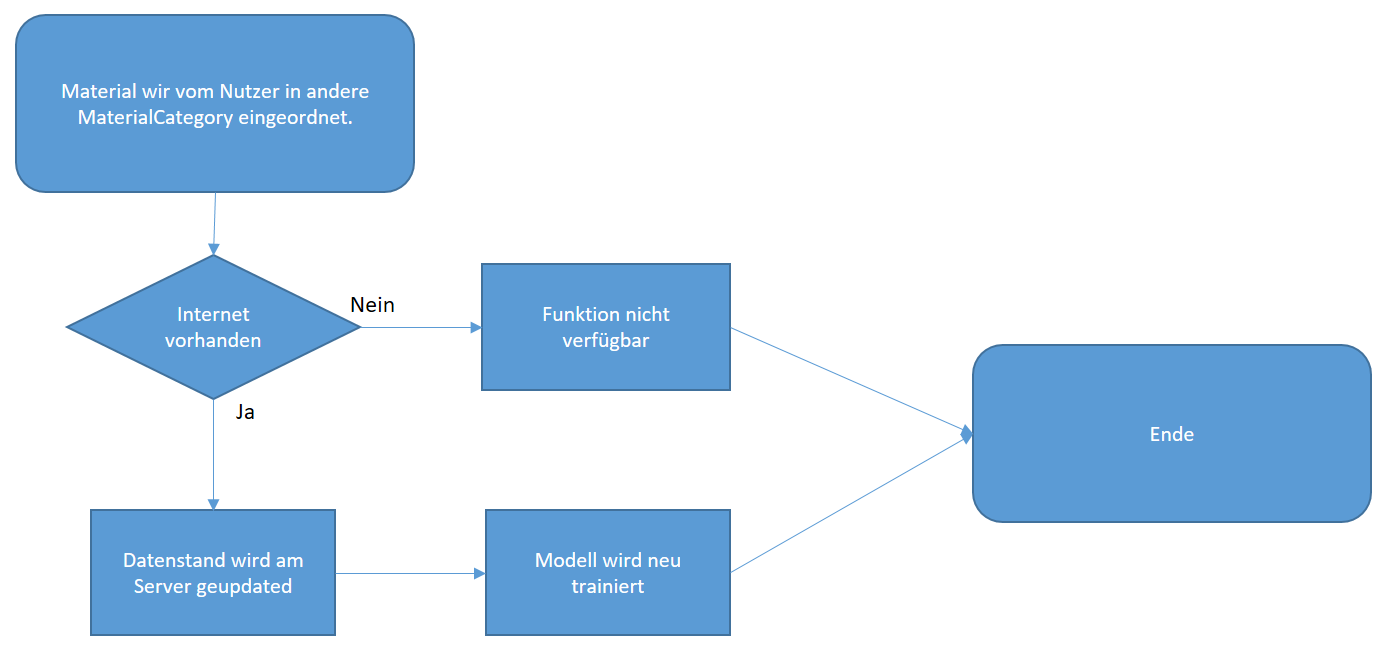
\includegraphics[width=1\linewidth]{function-rating}
	\caption[Rating]{Flussdiagramm Bewertung des Kostengliederungs-Import}
	\label{fig:func-rating}
\end{figure}

\begin{figure}[H]
	\centering
	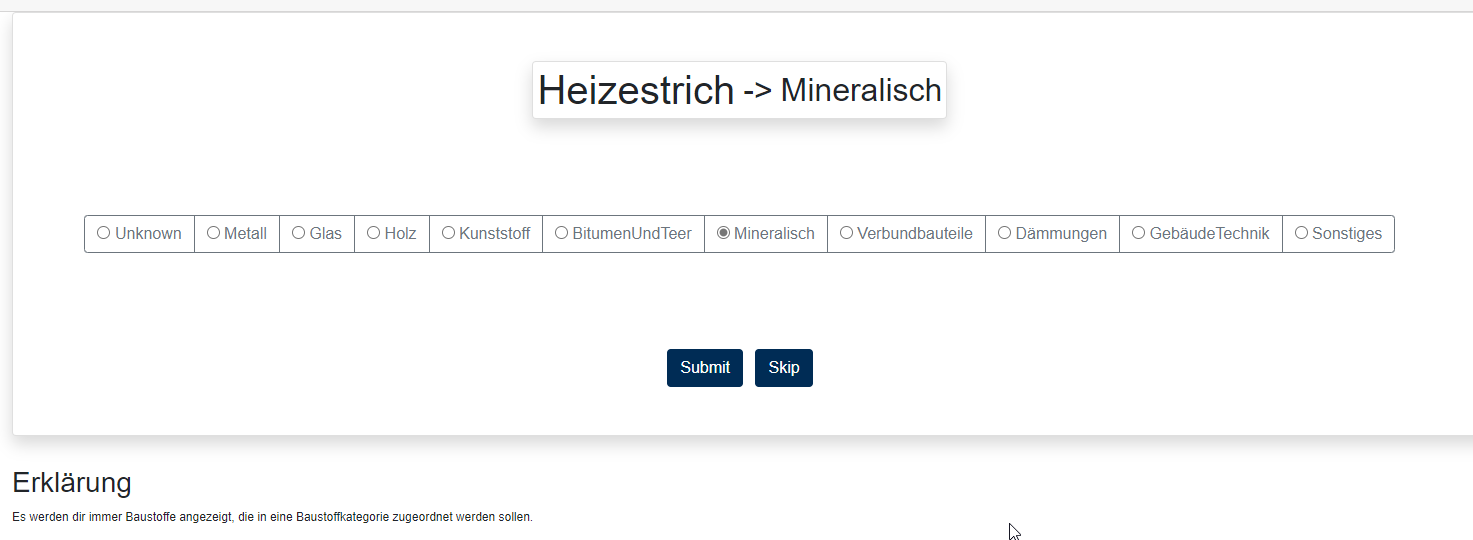
\includegraphics[width=1\linewidth]{material-classifier-gui}
	\caption[Rating]{Oberfläche des Klassifizierungs-Tools für Materialien}
	\label{fig:classification-service}
\end{figure}

\section*{Listings}
\label{c:listings}

\lstinputlisting[language={[Sharp]C}, caption={Implementierung der Methode \code{GenerateMaterialCostStructureAsync} der Klasse \code{MateialService}}, style={csharp}, label={lst:materialservice}]{MaterialService.cs}

\lstinputlisting[language={[Sharp]C}, caption={Python-Interopt für das Preprocessing}, style={csharp}, label={lst:python-preprocess}]{PythonPreprocess.cs}

\lstinputlisting[language={python}, caption={Python-Interopt für das Preprocessing}, label={Script}, label={lst:preprocess}]{preprocess.py}

\section*{Tabellen}
\label{c:tables}
\begin{table}[h]

	\centering
\begin{tabular}{|l|l|l|l|}
	\hline
	\textbf{Begriff} & \textbf{Erwartet} & \textbf{DBSCAN} & \textbf{OpenAI}\\ \hline
   Ortbeton C30/37 Verputzt & 1 & 1 & ~ \\ \hline
Trockenbau Gipsplatte & ~ & ~ & ~ \\ \hline
Fußboden Heizestrich & 3 & 3 & 3 \\ \hline
Geländearbeiten Gebundene Schüttung & 4 & 4 & 4 \\ \hline
Ortbeton C30/37 & 1 & 1 & ~ \\ \hline
Mauerwerk mit Daemmeigenschaften & 2 & 2 & 2 \\ \hline
Fußboden Fußbodenaufbau & 3 & 3 & 3 \\ \hline
Fußboden Schüttung & 3 & ~ & 3 \\ \hline
Putz & ~ & ~ & ~ \\ \hline
Geländearbeiten Rollierung Schuettung & 4 & 4 & 4 \\ \hline
Ortbeton bewehrt geschliffen & 1 & ~ & ~ \\ \hline
Geländearbeiten Aufgeschüttet & 4 & 4 & 4 \\ \hline
Fußboden Estrich & 3 & 3 & 3 \\ \hline
Beton C 25/30 & 1 & 1 & ~ \\ \hline
Dachdeckung Ziegel & ~ & ~ & ~ \\ \hline
Mauerwerk ohne Daemmeigenschaften & 2 & 2 & 2 \\ \hline
\textbf{Auswertung} & richtig & teilweise & teilweise \\ \hline
	\end{tabular}
	\caption{Evaluationsbeispiel 1 (Überkategorie: Mineralisch)}
	\label{t:evaluation-example1}
\end{table}

\begin{table}[h]
	
	\centering
	\begin{tabular}{|l|l|l|l|}
		\hline
		\textbf{Begriff} & \textbf{Erwartet} & \textbf{DBSCAN} & \textbf{OpenAI}\\ \hline
		 Keramik & ~ & ~ & ~ \\ \hline
		 Trockenbau Gipsplatte & 1 & 1 & 1 \\ \hline
		 Trockenbau Gipsplatte 2 & 1 & 1 & 1 \\ \hline
		 Trockenbau Gipsplatte 3 & 1 & 1 & 1 \\ \hline
		 Trockenbau Gipsplatte 4 & 1 & 1 & 1 \\ \hline
		 Fußboden Teppich & 2 & ~ & 2 \\ \hline
		 Fußboden Estrich & 2 & ~ & 2 \\ \hline
		 Fußboden Trittschall & 2 & 2 & 2 \\ \hline
		 Fußboden Schüttung & 2 & 2 & 2 \\ \hline
		 Geschossdecke FB 200 Fliese & 3 & 3 & ~ \\ \hline
		 Fußboden Fliese Travertin & 2 & 3 & 2 \\ \hline
		 Ortbeton bewehrt & 3 & ~ & ~ \\ \hline
		 Mauerwerk Ziegel \\ \hline
		\textbf{Auswertung} & richtig & falsch & teilweise \\ \hline
	\end{tabular}
	\caption{Evaluationsbeispiel 2 (Überkategorie: Mineralisch)}
	\label{t:evaluation-example2}
\end{table}

\begin{table}[h]
	
	\centering
	\begin{tabular}{|l|l|l|l|}
		\hline
		\textbf{Begriff} & \textbf{Erwartet} & \textbf{DBSCAN} & \textbf{OpenAI}\\ \hline
      	Gipskarton & ~ & ~ & ~ \\ \hline
		Keramik Fliesen & ~ & ~ & ~ \\ \hline
		Mauerwerk Betonblock & 1 & 1 & 1 \\ \hline
		Beton Gegossen & 2 & 2 & 2 \\ \hline
		Mauerwerk Ziegel & 1 & 1 & 1 \\ \hline
		Beton & 2 & 2 & 2 \\ \hline	
		\textbf{Auswertung} & richtig & richtig & richtig \\ \hline
	\end{tabular}
	\caption{Evaluationsbeispiel 3 (Überkategorie: Mineralisch)}
	\label{t:evaluation-example3}
\end{table}

\begin{table}[h]
	
	\centering
	\begin{tabular}{|l|l|l|l|}
		\hline
		\textbf{Begriff} & \textbf{Erwartet} & \textbf{DBSCAN} & \textbf{OpenAI}\\ \hline
		 Stütze Auflager & ~ & ~ & -1 \\ \hline
		Kalksandstein & ~ & ~ & ~ \\ \hline
		Kies & ~ & ~ & ~ \\ \hline
		Fliesen & ~ & ~ & 2 \\ \hline
		Estrich & ~ & ~ & 2 \\ \hline
		Gipsputz & ~ & ~ & ~ \\ \hline
		Volkernplatte & ~ & ~ & 1 \\ \hline
		Ausbauplatte GKBI & 1 & 1 & 1 \\ \hline
		Ausbauplatte GKB & 1 & 1 & 1 \\ \hline
		\textbf{Auswertung} & richtig & richtig & falsch \\ \hline
	\end{tabular}
	\caption{Evaluationsbeispiel 4 (Überkategorie: Mineralisch)}
	\label{t:evaluation-example4}
\end{table}

\begin{table}[h]
	
	\centering
	\begin{tabular}{|l|l|l|l|}
		\hline
		\textbf{Begriff} & \textbf{Erwartet} & \textbf{DBSCAN} & \textbf{OpenAI}\\ \hline
		 WI KS 17 5 & 1 & 1 & ~ \\ \hline
		Kalksandstein & 1 & ~ & 1 \\ \hline
		WI KS 11 5 & 1 & 1 & 1 \\ \hline
		DA Flachdach Kiesschicht & 3 & ~ & ~ \\ \hline
		Kies & 3 & ~ & ~ \\ \hline
		Fliesen & ~ & ~ & 3 \\ \hline
		Estrich & ~ & ~ & 3 \\ \hline
		Gipsputz & ~ & ~ & ~ \\ \hline
		Ausbauplatte GKBI & 2 & 2 & 2 \\ \hline
		Ausbauplatte GKB & 2 & 2 & 2 \\ \hline
		\textbf{Auswertung} & richtig & teilweise & falsch \\ \hline
	\end{tabular}
	\caption{Evaluationsbeispiel 5 (Überkategorie: Mineralisch)}
	\label{t:evaluation-example5}
\end{table}

\begin{table}[h]
	
	\centering
	\begin{tabular}{|l|l|l|l|}
		\hline
		\textbf{Begriff} & \textbf{Erwartet} & \textbf{DBSCAN} & \textbf{OpenAI}\\ \hline
		  Mauerwerk Langlochziegel verputzt & 1 & 1 & 1 \\ \hline
		Mauerwerk Ziegel verputzt & 1 & 1 & 1 \\ \hline
		MW Kalksandstein verputzt & 1 & 1 & 1 \\ \hline
		Knauf Bauplatte Typ A & ~ & ~ & ~ \\ \hline
		Decke Fliesen & ~ & ~ & ~ \\ \hline
		Beton Estrich & ~ & ~ & ~ \\ \hline
		Porenbeton verputzt & 1 & 1 & ~ \\ \hline
		Vorgabe Dach & ~ & ~ & ~ \\ \hline
		\textbf{Auswertung} & richtig & richtig & teilweise \\ \hline
	\end{tabular}
	\caption{Evaluationsbeispiel 6 (Überkategorie: Mineralisch)}
	\label{t:evaluation-example6}
\end{table}

\begin{table}[h]
	
	\centering
	\begin{tabular}{|l|l|l|l|}
		\hline
		\textbf{Begriff} & \textbf{Erwartet} & \textbf{DBSCAN} & \textbf{OpenAI}\\ \hline
		 A W TR MW KS 17 5 & 4 & 4 & ~ \\ \hline
		FAS PUTZ TYP1 0 2 0 & 1 & 1 & ~ \\ \hline
		I BOD ESTRICH ZE 6 & 2 & 2 & 2 \\ \hline
		I BOD ESTRICH ZE 7 & 2 & 2 & 2 \\ \hline
		FAS PUTZ TYP1 0 2 & 1 & 1 & ~ \\ \hline
		I BOD BELAG BETONSTEIN 3 & 3 & 3 & 3 \\ \hline
		I BOD ESTRICH ZE 4 & 2 & 2 & 2 \\ \hline
		I BOD BELAG FLIESE 1 5 & 3 & 3 & 3 \\ \hline
		I BOD ESTRICH ZE 5 5 & 2 & 2 & 2 \\ \hline
		I W TR MW KS 11 5 & 4 & 4 & ~ \\ \hline
		A BOD KIES 5 & ~ & ~ & ~ \\ \hline
		Gefällebeton & 5 & ~ & ~ \\ \hline
		Beton & 5 & ~ & ~ \\ \hline
		Concrete & 5 & ~ & ~ \\ \hline
		\textbf{Auswertung} & richtig & teilweise & teilweise \\ \hline
	\end{tabular}
	\caption{Evaluationsbeispiel 7 (Überkategorie: Mineralisch)}
	\label{t:evaluation-example7}
\end{table}

\begin{table}[h]
	
	\centering
	\begin{tabular}{|l|l|l|l|}
		\hline
		\textbf{Begriff} & \textbf{Erwartet} & \textbf{DBSCAN} & \textbf{OpenAI}\\ \hline
		        Metall Edelstahl gebürstet & 1 & 1 & 1 \\ \hline
		Fensterbank Aussen Blech & ~ & ~ & -1 \\ \hline
		Metall Edelstahl Satiniert & 1 & 1 & 1 \\ \hline
		Metall Stahl matt & ~ & 1 & ~ \\ \hline
		\textbf{Auswertung} & richtig & falsch & falsch \\ \hline
	\end{tabular}
	\caption{Evaluationsbeispiel 8 (Überkategorie: Metall)}
	\label{t:evaluation-example8}
\end{table}

\begin{table}[h]
	
	\centering
	\begin{tabular}{|l|l|l|l|}
		\hline
		\textbf{Begriff} & \textbf{Erwartet} & \textbf{DBSCAN} & \textbf{OpenAI}\\ \hline
		   Metall Titanzink & ~ & 2 & ~ \\ \hline
		Metall Oberfläche lackiert elfenbein Mit Glaz & 1 & 1 & 1 \\ \hline
		Metall Oberfläche lackiert matt & 1 & 1 & 1 \\ \hline
		Metall Aluminium & ~ & 2 & ~ \\ \hline
		Metall lackiert & 1 & 1 & ~ \\ \hline
		Metall verzinkt & ~ & 2 & ~ \\ \hline
		\textbf{Auswertung} & richtig & richtig & teilweise \\ \hline
	\end{tabular}
	\caption{Evaluationsbeispiel 9 (Überkategorie: Metall)}
	\label{t:evaluation-example9}
\end{table}

\begin{table}[h]
	
	\centering
	\begin{tabular}{|l|l|l|l|}
		\hline
		\textbf{Begriff} & \textbf{Erwartet} & \textbf{DBSCAN} & \textbf{OpenAI}\\ \hline
		  Metall Edelstahl Satiniert & 1 & 1 & 1 \\ \hline
		Metall Edelstahl gebürstet & 1 & 1 & 1 \\ \hline
		Metall Stahl matt & 2 & 1 & ~ \\ \hline
		Metal Strugal Stainless Steel & 1 & 2 & ~ \\ \hline
		Aluminum Strugal RAL 9016 & ~ & 2 & ~ \\ \hline
		Fensterbank Aussen Blech & ~ & 2 & ~ \\ \hline
		\textbf{Auswertung} & richtig & falsch & teilweise \\ \hline
	\end{tabular}
	\caption{Evaluationsbeispiel 10 (Überkategorie: Metall)}
	\label{t:evaluation-example10}
\end{table}

\begin{table}[h]
	
	\centering
	\begin{tabular}{|l|l|l|l|}
		\hline
		\textbf{Begriff} & \textbf{Erwartet} & \textbf{DBSCAN} & \textbf{OpenAI}\\ \hline
		 StB C45 & 1 & 1 & 1 \\ \hline
		StB C55 & 1 & 1 & 1 \\ \hline
		StB C35 & 1 & 1 & 1 \\ \hline
		StB C30 & 1 & 1 & 1 \\ \hline
		StB C60 & 1 & 1 & 1 \\ \hline
		Fertigteil StB C35 & 1 & 1 & 1 \\ \hline
		StB FU & 1 & ~ & 1 \\ \hline
		\textbf{Auswertung} & richtig & teilweise & richtig \\ \hline
	\end{tabular}
	\caption{Evaluationsbeispiel 11 (Überkategorie: Verbundbauteil)}
	\label{t:evaluation-example11}
\end{table}

\begin{table}[h]
	
	\centering
	\begin{tabular}{|l|l|l|l|}
		\hline
		\textbf{Begriff} & \textbf{Erwartet} & \textbf{DBSCAN} & \textbf{OpenAI}\\ \hline
		 Aluminium & ~ & ~ & ~ \\ \hline
		Stahl verzinkt & ~ & ~ & ~ \\ \hline
		Edelstahl  & ~ & ~ & ~ \\ \hline
		\textbf{Auswertung} & richtig & richtig & richtig\\ \hline
	\end{tabular}
	\caption{Evaluationsbeispiel 12 (Überkategorie: Metall)}
	\label{t:evaluation-example12}
\end{table}

\begin{table}[h]
	
	\centering
	\begin{tabular}{|l|l|l|l|}
		\hline
		\textbf{Begriff} & \textbf{Erwartet} & \textbf{DBSCAN} & \textbf{OpenAI}\\ \hline
		  DA Flachdach Gefälledämmung & 2 & 2 & 1 \\ \hline
		Mineralwolle 4 & 1 & 1 & 1 \\ \hline
		WA XPS Dämmung 10cm & 3 & ~ & 1 \\ \hline
		XPS & 3 & 2 & 1 \\ \hline
		DA Flachdach Dämmung 14cm & 2 & 2 & 1 \\ \hline
		Mineralwolle 3 & 1 & 1 & 1 \\ \hline
		Brandriegel & ~ & ~ & ~ \\ \hline
		Trittschalldämmung  & ~ & ~ & ~ \\ \hline
		\textbf{Auswertung} & richtig & falsch & falsch \\ \hline
	\end{tabular}
	\caption{Evaluationsbeispiel 13 (Überkategorie: Dämmungen)}
	\label{t:evaluation-example13}
\end{table}

\begin{table}[h]
	
	\centering
	\begin{tabular}{|l|l|l|l|}
		\hline
		\textbf{Begriff} & \textbf{Erwartet} & \textbf{DBSCAN} & \textbf{OpenAI}\\ \hline
		   DA Flachdach Dämmung 14cm & 3 & 2 & 1 \\ \hline
		Mineralwolle 3 & 1 & 1 & 1 \\ \hline
		WA XPS Dämmung 10cm & 2 & 2 & 1 \\ \hline
		XPS & 2 & ~ & 1 \\ \hline
		DA Flachdach Gefälledämmung & 3 & 2 & 1 \\ \hline
		Mineralwolle 4 & 1 & 1 & 1 \\ \hline
		Trittschalldämmung & ~ & ~ & ~ \\ \hline
		Brandriegel  & ~ & ~ & ~ \\ \hline
		\textbf{Auswertung} & richtig & falsch & falsch \\ \hline
	\end{tabular}
	\caption{Evaluationsbeispiel 14 (Überkategorie: Dämmungen)}
	\label{t:evaluation-example14}
\end{table}

\begin{table}[h]
	
	\centering
	\begin{tabular}{|l|l|l|l|}
		\hline
		\textbf{Begriff} & \textbf{Erwartet} & \textbf{DBSCAN} & \textbf{OpenAI}\\ \hline
		  FAS WDVS WD EPS 8 & 1 & 1 & 1 \\ \hline
		FAS WDVS WD EPS 18 & 1 & 1 & 1 \\ \hline
		I BOD DAEM TD 3 & ~ & ~ & 2 \\ \hline
		I BOD DAEM WD 14 & 2 & 2 & 2 \\ \hline
		I BOD DAEM WD 15 & 2 & 2 & 2 \\ \hline
		A BOD DAEM XPS 11 & 4 & 4 & 4 \\ \hline
		A W NT DAEM PD XPS 12 & 3 & 3 & 3 \\ \hline
		A W NT DAEM PD XPS 6 & 3 & 3 & 3 \\ \hline
		A BOD DAEM XPS 12 & 4 & 4 & 4 \\ \hline
		A BOD DAEM XPS 10 & 4 & 4 & 4 \\ \hline
		\textbf{Auswertung} & richtig & richtig & teilweise \\ \hline
	\end{tabular}
	\caption{Evaluationsbeispiel 15 (Überkategorie: Dämmungen)}
	\label{t:evaluation-example15}
\end{table}

\begin{table}[h]
	
	\centering
	\begin{tabular}{|l|l|l|l|}
		\hline
		\textbf{Begriff} & \textbf{Erwartet} & \textbf{DBSCAN} & \textbf{OpenAI}\\ \hline
		Glas Isolierverglasung klar & 1 & 1 & 1 \\ \hline
		Glas Isolierverglasung 3 fach & 1 & 2 & 1 \\ \hline
		Glas Isolierverglasung 2 fach & 1 & 2 & 1 \\ \hline
		Glas klar & 1 & 1 & ~ \\ \hline
		Glas matt & ~ & ~ & ~ \\ \hline
		\textbf{Auswertung} & richtig & falsch & teilweise\\ \hline
	\end{tabular}
	\caption{Evaluationsbeispiel 16 (Überkategorie: Glas)}
	\label{t:evaluation-example16}
\end{table}

\begin{table}[h]
	
	\centering
	\begin{tabular}{|l|l|l|l|}
		\hline
		\textbf{Begriff} & \textbf{Erwartet} & \textbf{DBSCAN} & \textbf{OpenAI}\\ \hline
		Glas matt & ~ & ~ & ~ \\ \hline
		Glas Isolierverglasung Bronze & 1 & ~ & 1 \\ \hline
		Glass Strugal Clear Glazing & 1 & 2 & ~ \\ \hline
		Glas klar & 1 & 1 & ~ \\ \hline
		Glass Simonton Clear & 1 & 2 & ~ \\ \hline
		Glas Isolierverglasung klar & 1 & 1 & 1 \\ \hline
		\textbf{Auswertung} & richtig & falsch & teilweise \\ \hline
	\end{tabular}
	\caption{Evaluationsbeispiel 17 (Überkategorie: Glas)}
	\label{t:evaluation-example17}
\end{table}

\begin{table}[h]
	
	\centering
	\begin{tabular}{|l|l|l|l|}
		\hline
		\textbf{Begriff} & \textbf{Erwartet} & \textbf{DBSCAN} & \textbf{OpenAI}\\ \hline
		 Geschossdecke FB 200 Parkett & 2 & 2 & -1 \\ \hline
		 Holz generisch & ~ & 1 & ~ \\ \hline
		 Fußboden Parkett eiche & 2 & 2 & -1 \\ \hline
		 Dachdeckung Holz & 1 & 1 & 1 \\ \hline
		 Dachdeckung Holz 2 & 1 & 1 & 1 \\ \hline
		\textbf{Auswertung} & richtig & teilweise & falsch \\ \hline
	\end{tabular}
	\caption{Evaluationsbeispiel 18 (Überkategorie: Holz)}
	\label{t:evaluation-example18}
\end{table}

\begin{table}[h]
	
	\centering
	\begin{tabular}{|l|l|l|l|}
		\hline
		\textbf{Begriff} & \textbf{Erwartet} & \textbf{DBSCAN} & \textbf{OpenAI}\\ \hline
		 Holz Parkett & ~ & ~ & 1 \\ \hline
		Holz Birke & 1 & 1 & 1 \\ \hline
		Holz Eiche & 1 & 1 & 1 \\ \hline
		Standard Treppe & ~ & ~ & ~ \\ \hline
		\textbf{Auswertung} & richtig & richtig & teilweise \\ \hline
	\end{tabular}
	\caption{Evaluationsbeispiel 19 (Überkategorie: Holz)}
	\label{t:evaluation-example19}
\end{table}

\begin{table}[h]
	
	\centering
	\begin{tabular}{|l|l|l|l|}
		\hline
		\textbf{Begriff} & \textbf{Erwartet} & \textbf{DBSCAN} & \textbf{OpenAI}\\ \hline
		  Dachdeckung Holz & ~ & ~ & ~ \\ \hline
		Fußboden Terrasse Teakholz & ~ & ~ & ~ \\ \hline
		Holz HSB Steher & ~ & ~ & ~ \\ \hline
		Holz Astfichte senkrecht & ~ & ~ & ~ \\ \hline
		\textbf{Auswertung} & richtig & richtig & richtig \\ \hline
	\end{tabular}
	\caption{Evaluationsbeispiel 20 (Überkategorie: Holz)}
	\label{t:evaluation-example20}
\end{table}

\begin{table}[h]
	
	\centering
	\begin{tabular}{|l|l|l|l|}
		\hline
		\textbf{Begriff} & \textbf{Erwartet} & \textbf{DBSCAN} & \textbf{OpenAI}\\ \hline
		 Fußboden Epoxidharzbeschichtung & ~ & ~ & ~ \\ \hline
		BSt 500 M A & 1 & 1 & 1 \\ \hline
		BSt 500 M B & 1 & 1 & 1 \\ \hline
		\textbf{Auswertung} & richtig & richtig & richtig\\ \hline
	\end{tabular}
	\caption{Evaluationsbeispiel 21 (Überkategorie: Verbundbauteile)}
	\label{t:evaluation-example21}
\end{table}

\begin{table}[h]
	
	\centering
	\begin{tabular}{|l|l|l|l|}
		\hline
		\textbf{Begriff} & \textbf{Erwartet} & \textbf{DBSCAN} & \textbf{OpenAI}\\ \hline
		  A W TR STB OB 17 5 & 1 & 1 & -1 \\ \hline
		I W TR STB OB 25 & 1 & 2 & -1 \\ \hline
		A DE TR STB OB 30 & 3 & ~ & -1 \\ \hline
		I W TR STB OB 12 & 1 & 2 & -1 \\ \hline
		A W TR STB OB 25 & 1 & 1 & -1 \\ \hline
		A W TR STB OB 30 & 1 & 1 & -1 \\ \hline
		I W TR STB OB 22 & 1 & 2 & -1 \\ \hline
		I DE TR STB OB 20 & 3 & 3 & -1 \\ \hline
		I DE TR STB OB 45 & 3 & 3 & -1 \\ \hline
		I DE TR STB OB 25 & 3 & 3 & -1 \\ \hline
		\textbf{Auswertung} & richtig & teilweise & teilweise \\ \hline
	\end{tabular}
	\caption{Evaluationsbeispiel 22 (Überkategorie: Verbundbauteile)}
	\label{t:evaluation-example22}
\end{table}





\cleardoublepage

\begin{acronym}

\acro{ifc}[IFC]{Industy Foundation Classes}
\acro{ifc2x3}[IFC2x3]{\ac{ifc} Version 2.3}
\acro{ifc4}[IFC4]{\ac{ifc} Version 4}
\acro{bim}[BIM]{Building Information Modeling}

\end{acronym}
\cleardoublepage

\stepcounter{chapter} %increment counter of chapters B -> C
\def\verzeichnisdef{\Alph{chapter} ~~} %variable

\addcontentsline{toc}{chapter}{\verzeichnisdef Definitionsverzeichnis}

\listoftheorems[ignore={goal,problem,requirement},show={definition},title={\verzeichnisdef Definitionsverzeichnis}]

\stepcounter{chapter} %increment counter of chapters C -> D
\def\listingdef{\Alph{chapter} ~~} %variable

\addcontentsline{toc}{chapter}{\listingdef Quellcodeverzeichnis}

\renewcommand{\lstlistlistingname}{\listingdef Quellcodeverzeichnis}
\lstlistoflistings

\printindex

\end{document}